\actTitle{1.8 - Algebra of Functions and Function Composition}

\videoLink{Section 1.8}{https://www.youtube.com/playlist?list=PLYHZK3b8UFw2GleEiLibLzFIsnrHdy43\_}

\noindent \textbf{Topics:}  basic operations on functions, composition of functions, and difference quotient\\

\noindent \textbf{Student Learning Outcomes:}
\begin{enumerate}
\item Students will be able to perform basic operations on functions.
\item Students will be able to compose functions.
\item Students will be able to evaluate a difference quotient.
\end{enumerate}

\hrule 

\bigskip

\subsection{Algebra on Functions}


\begin{enumerate}
\item Find the following values for the functions $f(x) = x + 3$ and $g(x) = x^2$.
\begin{enumerate}
\item $(f+g)(2)$ \vfill 
\item $(f-g)(7)$ \vfill
\item $(fg)(5)$ \\(same as $(f\cdot g )(5)$)\vfill
\item $(f/g)(4)$\vfill
\end{enumerate}




\newpage


\subsection{Function Composition}
The composition of two functions, $f(x)$ and $g(x)$, is given by
	$$(f \circ g)(x)=f[g(x)] \quad \quad \text{or} \quad \quad (g \circ f)(x)=g[f(x)]$$
that is, by "plugging one function into another". One must be careful, however, as the above two quantities are \textbf{\underline{not equal}} in general (it is also important not to confuse this notation with multiplying two functions, hence the use of the "open circle" symbol).

\item Find the following values for the functions $f(x) = x + 3$ and $g(x) = x^2$.
\begin{enumerate}
\item $f(g(4))$\\[1in]
\item $g(f(4))$\\[1in]

\end{enumerate}


\item Use $f(x) = \dfrac{1}{3-x}$ and $g(x)=3x^2-16$ to answer the following.
\begin{enumerate}
\item Determine $f(g(x))$ and the domain of $f(g(x))$. \\[1in]
\item Determine $(g \circ f)(x)$ and the domain of $(g \circ f)(x)$. \\[1in]
%\item Determine $(g \circ g)(x)$. \\ \\ 

\item Determine $g(f(3))$. \\ \\
\end{enumerate}



\newpage

\item \textbf{Decomposition}  Find functions $f$, $g$, such that $f(g(x))=y$ for the function $y = 6 + \sqrt{9-x^2}$. (There is more than one correct answer.) \\[1in]

\item Use the graphs of $f$ and $g$ below to determine the following.
\begin{enumerate}
\item $f (g(2))$  \\[.5in] 
\item $g(f(4))$  \\[.5in] 
\item $f(g(1))$ \\[.5in] 

\end{enumerate}


\noindent \scalebox{1}{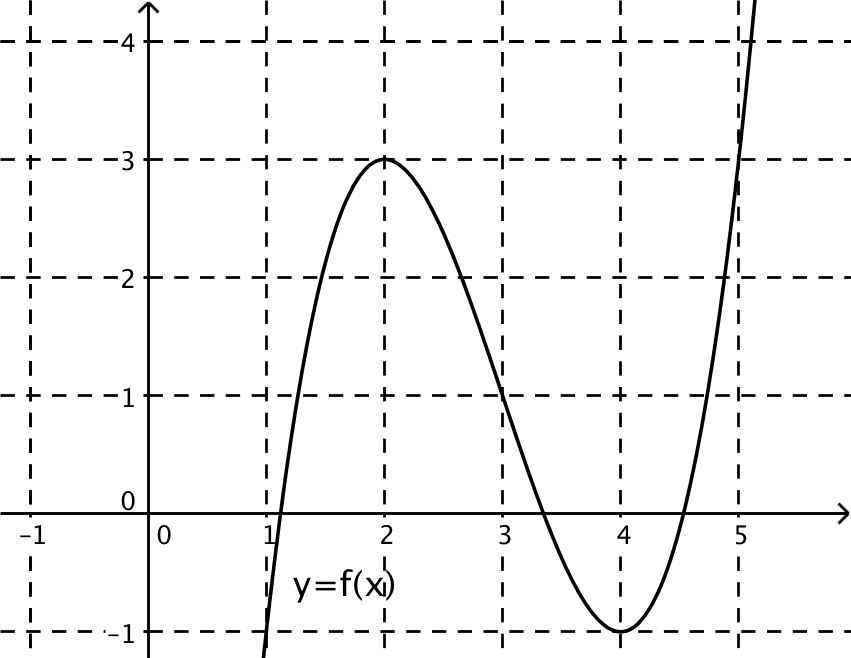
\includegraphics{comp1}} \hspace{1in} \scalebox{1}{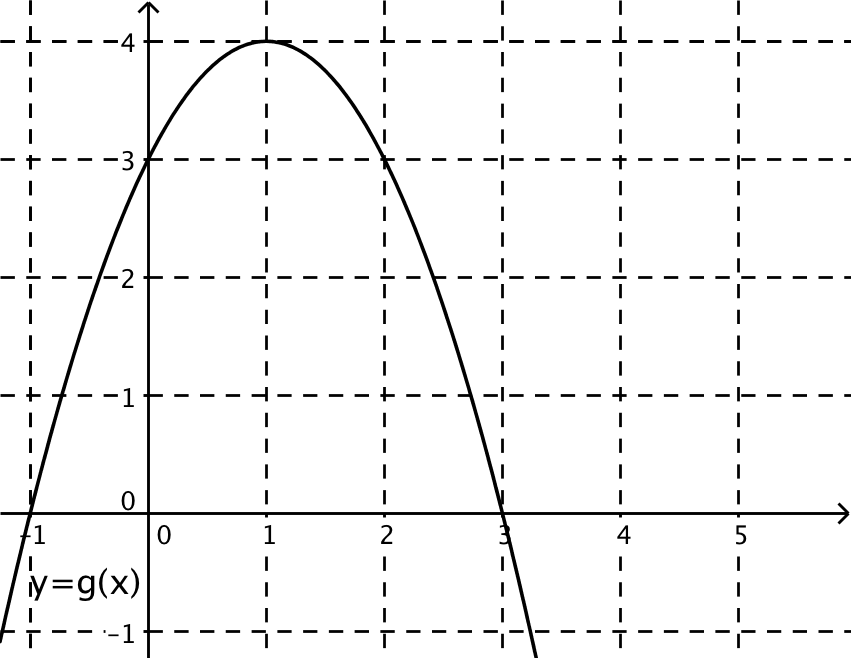
\includegraphics{comp2}}

\newpage

\subsection{Diference Quotient}

\textbf{Recall:}The slope of a line through two points $(x_1, y_1)$ and $(x_2, y_2)$ is given by the formula
$$m=\frac{y_2-y_1}{x_2-x_1}=\frac{\Delta y}{\Delta x}=\frac{\text{change in y}}{\text{change in x}}$$


\textbf{Average Rate of Change}\\


 The \textbf{\emph{average rate of change}} of $y=f(x)$ with respect to $x$ over the interval $[x_1,x_2]$ is
 $$\frac{\Delta y}{\Delta x}=\frac{f(x_2)-f(x_1)}{x_2-x_1}=\frac{f(x_1+h)-f(x_1)}{h}, h\neq 0.$$\\ 
 
 This is the \textbf{difference quotient.}  Let's draw a graph.
 \vfill
 
 \item Given $f(x)=3x-5$.
 \begin{enumerate}
 \item Find $f(x+h)$.\\[.5in]
 \item Find the difference quotient, $\frac{f(x+h)-f(x)}{h}$.\\[1.5in]
 \end{enumerate}





\end{enumerate}

\noindent \textbf{Student Learning Outcomes Check}

\begin{enumerate}
\item Can you perform basic algebra operations on functions?
\item Can you compose functions two functions?
\item Are you able to evaluate a difference quotient?


\end{enumerate}

\noindent \textbf{If any of your answers were no, please ask about these topics in class.}


